\chapter{NLP}\label{NLP}
Nell'era dell'informazione digitale, il trattamento del linguaggio naturale (NLP) ha acquisito un ruolo di primaria importanza, ponendo le basi per l'interazione senza soluzione di continuità tra esseri umani e macchine attraverso il linguaggio. La capacità di comprendere, interpretare e generare il linguaggio umano non solo rappresenta un trampolino per l'efficienza nelle comunicazioni, ma costituisce anche un cardine fondamentale per l'automazione delle attività cognitive e la creazione di sistemi intelligenti.

Questa capitolo esplora le profondità del NLP, un campo interdisciplinare che fonde la linguistica, l'informatica e l'apprendimento automatico al fine di consentire alle macchine di cogliere le sfumature e le complessità del linguaggio umano, esploreremo inizialmente il concetto stesso di NLP, gettando le basi per una comprensione più approfondita delle sue sfaccettature. Saranno affrontate le sue applicazioni pervasive in vari settori, dimostrando come il NLP giochi un ruolo chiave nella traduzione automatica, nell'analisi dei sentimenti, nell'interazione uomo-macchina e in molte altre aree cruciali.

Tuttavia, il NLP non è privo di sfide. L'ambiguità del linguaggio, la variazione linguistica e la comprensione del contesto rappresentano ostacoli significativi che richiedono soluzioni innovative.

Inoltre, un aspetto centrale del mondo NLP è rappresentato dagli ``embedding'' di parole, che fungono da ponte tra il mondo del linguaggio umano e quello dell'apprendimento automatico. Approfondiremo il concetto di embedding e analizzeremo alcune delle tecniche di generazione degli stessi, con particolare attenzione all'algoritmo Word2Vec e alla sua rilevanza nell'elaborazione del linguaggio naturale.

Infine, daremo uno sguardo ai database vettoriali, strumenti essenziali per l'indicizzazione e il recupero efficiente delle informazioni nei vasti corpus di testo. Esamineremo come queste strutture dati permettano di navigare attraverso l'oceano di dati testuali con una precisione e una rapidità senza precedenti.
\section{Cos'è il NLP}
Il Trattamento del Linguaggio Naturale (Natural Language Processing, NLP) è un campo interdisciplinare che si situa all'intersezione tra la linguistica computazionale, l'informatica e l'apprendimento automatico. L'obiettivo fondamentale del NLP è quello di consentire alle macchine di comprendere, interpretare e generare il linguaggio umano in modi che risultino naturali e significativi per gli esseri umani stessi. In altre parole, il NLP mira a colmare il divario tra il linguaggio naturale, che è intrinsecamente complesso e vario, e le rappresentazioni numeriche manipolabili dalle macchine.

La centralità del NLP nel contesto dell'evoluzione tecnologica moderna è palese. Da chatbot interattivi a motori di ricerca avanzati, da assistenti vocali a sistemi di traduzione istantanea, il NLP è diventato la spina dorsale dell'interazione tra esseri umani e computer. Attraverso l'analisi e l'elaborazione dei testi scritti e delle conversazioni vocali, il NLP rende possibile l'automazione di molte attività cognitive, offrendo opportunità innovative in una vasta gamma di settori.

Uno dei pilastri del NLP è la capacità di analizzare e comprendere il significato del linguaggio umano. Questo va ben oltre la mera decodifica delle parole; coinvolge la comprensione delle strutture grammaticali, delle sfumature semantiche, dei contesti culturali e delle espressioni idiomatiche. Il NLP cerca di scomporre il linguaggio in componenti comprensibili per le macchine, creando così le basi per una comunicazione significativa.

Un aspetto cruciale del NLP è la bidirezionalità dell'interazione. Non solo le macchine devono essere in grado di comprendere il linguaggio umano, ma devono anche essere in grado di comunicare in modo efficace con gli esseri umani. Ciò richiede la generazione di testo naturale, un compito altrettanto complesso che coinvolge la scelta di parole appropriate, la coerenza del contesto e la produzione di espressioni coerenti.

In sintesi, il NLP è un campo che ha rivoluzionato la nostra capacità di interagire con le macchine attraverso il linguaggio naturale. La sua portata si estende dalle applicazioni pratiche che affrontiamo quotidianamente, come l'assistenza virtuale, alla ricerca accademica che cerca di comprendere le sfumature più profonde della comunicazione umana. Nel prosieguo di questo capitolo, esploreremo le applicazioni del NLP e come le sue tecniche si sono evolute per rispondere alle sfide poste dalla complessità del linguaggio umano.


\section{Le applicazioni del NLP}
Il Trattamento del Linguaggio Naturale (Natural Language Processing, NLP) ha rivoluzionato il modo in cui interagiamo con la tecnologia e ha aperto la strada a una vasta gamma di applicazioni che coinvolgono il linguaggio umano. Queste applicazioni, spesso impercettibili ma onnipresenti, spaziano dalla semplificazione delle nostre attività quotidiane alla rivoluzione di interi settori industriali. Di seguito, esploreremo alcune delle applicazioni chiave del NLP e il modo in cui esse influenzano la nostra vita quotidiana.

Traduzione automatica: Una delle prime applicazioni rivoluzionarie del NLP è stata la traduzione automatica. I sistemi di traduzione automatica consentono di superare le barriere linguistiche, consentendo alle persone di comunicare e comprendere contenuti in lingue diverse. Da servizi online a dispositivi mobili, la traduzione automatica è diventata un pilastro dell'interazione globale.

Analisi dei sentimenti: Il NLP ha reso possibile l'analisi dei sentimenti su larga scala, consentendo alle aziende di valutare le opinioni degli utenti attraverso i social media, le recensioni online e altri canali. Questa analisi consente alle imprese di ottenere una comprensione più profonda dell'opinione pubblica e di adattare le loro strategie di conseguenza.

Generazione di testo: L'NLP è alla base della generazione automatica di testo, che va dai suggerimenti di completamento nei messaggi di testo alla creazione di articoli giornalistici e contenuti online. I sistemi di generazione di testo possono produrre testi coerenti e pertinenti, offrendo un potenziale significativo per l'automazione di attività di scrittura.

Assistenti virtuali e chatbot: L'evoluzione degli assistenti virtuali come Siri, Google Assistant e Alexa è stata guidata dall'NLP. Questi assistenti virtuali sono in grado di rispondere a domande, fornire informazioni e eseguire compiti utilizzando il linguaggio naturale. Inoltre, i chatbot stanno diventando sempre più comuni nelle piattaforme di servizio clienti online, migliorando l'efficienza dell'interazione tra aziende e utenti.

Elaborazione del linguaggio naturale nei settori professionali: L'NLP è ampiamente utilizzato in ambito legale, medico e finanziario per analizzare grandi quantità di testi. Ad esempio, il NLP può essere utilizzato per analizzare documenti legali e trovare informazioni chiave, per estrarre informazioni mediche da report o per monitorare i mercati finanziari attraverso l'analisi dei notiziari.

Ricerca accademica e sviluppo tecnologico: L'NLP gioca un ruolo fondamentale nella ricerca accademica e nello sviluppo tecnologico. Dalla comprensione delle strutture linguistiche alla creazione di modelli avanzati di analisi semantica, il NLP apre nuove strade di esplorazione nel campo dell'intelligenza artificiale.

In sintesi, il NLP ha ampliato notevolmente la gamma di possibilità per l'interazione tra esseri umani e macchine attraverso il linguaggio. Le applicazioni del NLP sono varie e in continua espansione, plasmando l'evoluzione della nostra società digitale e aprendo nuovi orizzonti nei settori più diversi.
\section{Le problematiche del NLP}
Nonostante i progressi notevoli nel campo del Trattamento del Linguaggio Naturale (Natural Language Processing, NLP), ci sono sfide intrinseche che persistono a causa della complessità e dell'ambiguità del linguaggio umano. Queste problematiche rappresentano ostacoli che richiedono soluzioni innovative per consentire alle macchine di comprendere e generare il linguaggio in modo accurato.

Ambiguità linguistica: L'ambiguità è una caratteristica intrinseca del linguaggio umano, dove le stesse parole o frasi possono avere significati diversi a seconda del contesto. L'NLP deve affrontare l'ambiguità per garantire che le interpretazioni siano corrette e coerenti.

Variazione linguistica: Le lingue naturali presentano una vasta gamma di variazioni dialettali, regionali e culturali. L'NLP deve essere in grado di gestire queste variazioni per comprendere e generare testi che siano pertinenti per un pubblico globale e diversificato.

Comprensione del contesto: La comprensione del contesto è essenziale per una corretta interpretazione delle frasi. Le macchine devono essere in grado di cogliere il contesto circostante per evitare fraintendimenti e rispondere in modo appropriato.

Ironia e sfumature linguistiche: L'ironia, il sarcasmo e altre sfumature linguistiche rappresentano sfide particolari per l'NLP. Questi elementi richiedono una comprensione più profonda del significato implicito dietro le parole.

Mancanza di dati etichettati: L'addestramento di modelli NLP richiede una grande quantità di dati etichettati, ma talvolta questi dati possono essere limitati o costosi da ottenere. La mancanza di dati etichettati può influenzare la qualità delle prestazioni dei modelli.

Bias nel linguaggio: I dati utilizzati per addestrare i modelli NLP possono riflettere pregiudizi e stereotipi culturali. Di conseguenza, i modelli possono ereditare tali bias, portando a risultati ingiusti o discriminatori.

Sfide multilingue: L'elaborazione del linguaggio naturale in lingue diverse rappresenta sfide uniche a causa delle differenze linguistiche e culturali. I modelli NLP devono essere in grado di affrontare queste sfide per garantire risultati accurati e coerenti in tutto il mondo.

Privacy e sicurezza: L'elaborazione del linguaggio può coinvolgere la manipolazione di dati sensibili. La protezione della privacy e la sicurezza dei dati sono questioni cruciali nell'NLP, specialmente quando si tratta di conversazioni personali e informazioni confidenziali.

Affrontare queste problematiche richiede l'impiego di metodologie avanzate, come l'apprendimento profondo, insieme a un approccio etico e consapevole per mitigare il rischio di risultati distorti o dannosi. Nel prosieguo di questo capitolo, esploreremo alcune delle soluzioni proposte per affrontare tali sfide e per migliorare la precisione e l'efficacia delle applicazioni NLP.

\section{Le soluzioni del NLP}
Affrontare le sfide del Trattamento del Linguaggio Naturale (Natural Language Processing, NLP) richiede un approccio innovativo e multidisciplinare. Nel corso degli anni, la comunità di ricerca e gli sviluppatori hanno proposto una serie di soluzioni per mitigare le problematiche e migliorare l'efficacia delle applicazioni NLP. Di seguito, esploreremo alcune delle soluzioni chiave che stanno contribuendo a superare le sfide del NLP.
\begin{itemize}
    \item \textbf{Apprendimento profondo}: L'apprendimento profondo, o deep learning, è un paradigma di apprendimento automatico che ha dimostrato notevoli successi nell'NLP. Modelli come le reti neurali ricorrenti (RNN) e i transformer sono in grado di catturare le complessità del linguaggio, migliorando laccuratezza di comprensione e generazione del testo. Tuttavia, l'evoluzione dell'NLP non si è fermata qui. Negli ultimi anni, si è assistito a un'accelerazione delle ricerche che ha portato alla nascita di modelli ancora più avanzati. Tra questi, spiccano i modelli di linguaggio preaddestrati, come GPT (Generative Pre-trained Transformer) e BERT (Bidirectional Encoder Representations from Transformers), che hanno introdotto nuove prospettive nell'NLP. Questi modelli sfruttano grandi quantità di testo per imparare rappresentazioni linguistiche sempre più ricche, permettendo di cogliere sfumature e significati contestuali. L'approccio preaddestrato-codicificato-sintonizzato (pretrain-encode-tune) di questi modelli ha rivoluzionato il modo in cui affrontiamo molte sfide del NLP. Parallelamente all'innovazione dei modelli, la disponibilità di dati e risorse ha giocato un ruolo fondamentale nel superare le sfide del NLP. Grandi collezioni di testi multilingue e multimodali, insieme a dataset annotati specifici per compiti come la traduzione automatica, l'analisi del sentiment e l'estrazione delle informazioni, hanno alimentato l'allenamento e la valutazione dei modelli. Tuttavia, è emerso un nuovo set di sfide legate all'etica e alla privacy nell'uso di dati sensibili e all'ingiustizia nei dati di addestramento, che richiedono un'attenzione rigorosa per garantire l'equità nei risultati ottenuti.
    
    \item \textbf{Transfer learning}: Il transfer learning consiste nell'addestrare modelli NLP su grandi dataset generici e successivamente fine-tuning su task specifici con dataset più piccoli. Questo approccio consente di sfruttare la conoscenza pregressa del linguaggio per migliorare le prestazioni su task specifici.

    \item \textbf{Rappresentazioni vettoriali avanzate}: Le rappresentazioni vettoriali, come gli embedding di parole, sono fondamentali nell'NLP. Tecniche avanzate come Word2Vec, GloVe e BERT consentono di catturare relazioni semantiche complesse tra le parole, migliorando la comprensione del testo da parte delle macchine.

    \item \textbf{Augmentation dei dati}: L'augmentation dei dati è una tecnica che consiste nel generare dati sintetici a partire dai dati esistenti. Questo approccio può aumentare la diversità dei dati di addestramento e ridurre l'overfitting, migliorando la generalizzazione dei modelli.

    \item \textbf{Approcci basati su regole}: In alcune situazioni, l'uso di regole linguistiche specifiche può aiutare a gestire le ambiguità e a migliorare l'interpretazione del testo. Gli approcci basati su regole possono essere utili per affrontare problematiche specifiche e guidare l'elaborazione del linguaggio.

    \item \textbf{Mitigazione del bias}: Per affrontare il bias nel linguaggio, sono state proposte strategie di mitigazione, come l'analisi dei dati per identificare e correggere i bias presenti. È importante adottare un approccio etico nell'addestramento dei modelli NLP per evitare risultati discriminatori.

    \item \textbf{Sviluppo collaborativo e open-source}: La comunità di ricerca e sviluppo nell'NLP ha adottato un approccio collaborativo, condividendo dati, modelli e algoritmi open-source. Questo contribuisce a accelerare l'innovazione e a migliorare le soluzioni attraverso la collaborazione globale.
\end{itemize}
È importante notare che molte delle soluzioni proposte sono interconnesse e possono essere combinate per affrontare sfide complesse. Affrontare le problematiche del NLP richiede un approccio multidisciplinare e una comprensione approfondita delle dinamiche del linguaggio umano. Nel prosieguo di questo capitolo, ci concentreremo su una tecnica chiave per la creazione di rappresentazioni vettoriali avanzate: l'algoritmo Word2Vec.
\section{Cos'è un embedding}
Un concetto fondamentale nel Trattamento del Linguaggio Naturale (Natural Language Processing, NLP) è quello degli "embedding" di parole. Gli embedding sono rappresentazioni numeriche che catturano le caratteristiche semantiche delle parole o dei testi. Questi vettori numerici consentono alle macchine di elaborare il linguaggio naturale in termini comprensibili per i modelli di apprendimento automatico. Gli embedding hanno rivoluzionato il modo in cui le parole vengono trattate nell'NLP, consentendo la creazione di modelli che possono cogliere le relazioni semantiche tra le parole e le sfumature di significato.

Evoluzione delle rappresentazioni vettoriali
L'idea di rappresentare parole come vettori numerici ha radici nella linguistica computazionale degli anni '90. Tuttavia, la svolta nell'uso di embedding di parole è arrivata con l'avvento delle tecniche di apprendimento profondo. In particolare, l'algoritmo Word2Vec ha rivoluzionato il modo in cui le parole vengono codificate come vettori. Word2Vec è stato introdotto da Mikolov et al. nel 2013 ed è diventato un pilastro nell'NLP.

Word2Vec e apprendimento distribuito
Word2Vec è un modello di apprendimento automatico che genera embedding di parole basati sulla distribuzione delle parole nel contesto. L'idea centrale è che parole simili tendono ad apparire in contesti simili. Word2Vec offre due approcci principali: Continuous Bag of Words (CBOW) e Skip-gram. Nel modello CBOW, l'obiettivo è prevedere una parola dato il suo contesto, mentre nel modello Skip-gram, l'obiettivo è prevedere il contesto dati una parola. L'addestramento di Word2Vec consente di regolare i vettori in modo che le parole simili abbiano vettori simili.

Trasferimento di conoscenza e modelli pre-addestrati
Una delle chiavi per il successo delle rappresentazioni vettoriali come Word2Vec è la capacità di trasferire conoscenza. I modelli pre-addestrati possono essere utilizzati come punto di partenza per task specifici. Ad esempio, un modello Word2Vec addestrato su un ampio corpus può essere ulteriormente adattato per risolvere problemi specifici, come la classificazione di sentimenti o il riconoscimento di entità.

Oltre Word2Vec: Modelli Transformer
Negli anni successivi a Word2Vec, il campo ha visto un ulteriore avanzamento con l'introduzione dei modelli Transformer. Questi modelli, come BERT (Bidirectional Encoder Representations from Transformers), utilizzano un'architettura di auto-attenzione per catturare relazioni contestuali tra le parole in modo bidirezionale. Questi modelli hanno superato le prestazioni dei metodi precedenti in molte attività NLP, dimostrando l'importanza di modelli complessi e dati di addestramento su vasta scala.

Nel corso della sua evoluzione, il concetto di embedding ha cambiato radicalmente il modo in cui le parole vengono rappresentate e utilizzate nell'NLP. Dall'introduzione di Word2Vec all'ascesa dei modelli Transformer, le rappresentazioni vettoriali hanno alimentato l'innovazione e reso possibili progressi significativi nelle applicazioni NLP.
\section{Le tecniche di embedding}
Le tecniche di embedding costituiscono un pilastro essenziale nel Trattamento del Linguaggio Naturale (Natural Language Processing, NLP). Queste metodologie convertono le parole e i testi in rappresentazioni numeriche, consentendo alle macchine di trattare il linguaggio umano in formato comprensibile. Dall'introduzione di Word2Vec a soluzioni più avanzate come BERT e GPT, il campo delle tecniche di embedding ha segnato un'evoluzione significativa.

Word2Vec: Catturare il contesto
Word2Vec, introdotto da Mikolov et al. nel 2013, ha svolto un ruolo cruciale nell'evoluzione delle rappresentazioni vettoriali. Questa tecnica adotta un approccio basato sulla predizione del contesto: attraverso l'analisi delle parole circostanti, Word2Vec crea embedding che catturano le relazioni semantiche tra le parole. Questi embedding sono capaci di rappresentare sinonimi e relazioni tra parole simili.

GloVe: Combattere l'ambiguità
Il Global Vectors for Word Representation (GloVe) è un altro approccio popolare all'embedding di parole. Introdotto da Pennington et al. nel 2014, GloVe cerca di superare l'ambiguità linguistica basandosi sulla co-occorrenza delle parole. Questa tecnica considera la frequenza con cui due parole appaiono insieme nel testo, creando embedding che riflettono le relazioni statistiche tra le parole.

Modelli Transformer: Contesti complessi
L'introduzione dei modelli Transformer, con BERT e GPT in prima linea, ha segnato un'ulteriore avanzamento nel campo delle rappresentazioni vettoriali. Questi modelli si basano sull'architettura di auto-attenzione, consentendo loro di catturare relazioni contestuali complesse tra le parole. BERT, ad esempio, addestra una rete neurale a prevedere parole mancanti in una frase, generando embedding che riflettono una profonda comprensione del contesto.

Utilizzo dei modelli pre-addestrati
Un aspetto cruciale delle tecniche di embedding è l'uso di modelli pre-addestrati. Questi modelli, addestrati su grandi dataset, catturano una vasta gamma di relazioni linguistiche. I modelli pre-addestrati possono essere ulteriormente adattati a task specifici con un addestramento ulteriore, trasferendo così la conoscenza acquisita su task più generici a compiti più specializzati.

Applicazioni e impatto
Le tecniche di embedding hanno alimentato un'ampia gamma di applicazioni NLP, come l'analisi dei sentimenti, la traduzione automatica, la generazione di testo e molto altro. La loro capacità di catturare relazioni semantiche complesse ha rivoluzionato il modo in cui le macchine comprendono e producono il linguaggio naturale, aprendo la strada a nuove frontiere di interazione uomo-macchina.
\section{Word2Vec}
Word2Vec \cite{w2v} è un algoritmo di apprendimento automatico fondamentale nel campo del Trattamento del Linguaggio Naturale (Natural Language Processing, NLP). Introdotta da Mikolov et al. nel 2013, questa tecnica ha segnato una svolta nel modo in cui le parole vengono rappresentate come vettori numerici e come sono comprese le relazioni semantiche tra di loro. L'obiettivo principale di Word2Vec è di catturare la somiglianza semantica tra le parole, consentendo alle macchine di elaborare il linguaggio in modo significativo.

\subsubsection{La logica dietro Word2Vec}
Word2Vec sfrutta il principio di distribuzione del linguaggio naturale, che afferma che parole simili tendono a comparire nei medesimi contesti. L'algoritmo considera il contesto in cui le parole compaiono in un testo e cerca di rappresentare ogni parola in base al suo contesto di utilizzo. Questo processo cattura le relazioni semantiche tra le parole: parole simili avranno rappresentazioni simili.

\subsubsection{Continuous Bag of Words (CBOW) e Skip-gram}
Word2Vec offre due approcci principali: Continuous Bag of Words (CBOW) e Skip-gram. Nel modello CBOW, l'algoritmo cerca di prevedere una parola data una finestra di contesto, utilizzando il contesto per stimare la parola obiettivo. Nel modello Skip-gram, invece, l'obiettivo è prevedere il contesto (cioè le parole circostanti) data una parola. Entrambi gli approcci cercano di ottimizzare la capacità dell'algoritmo di rappresentare le parole in modo accurato.

\begin{center}
    \begin{figure}[H]
        \centering
        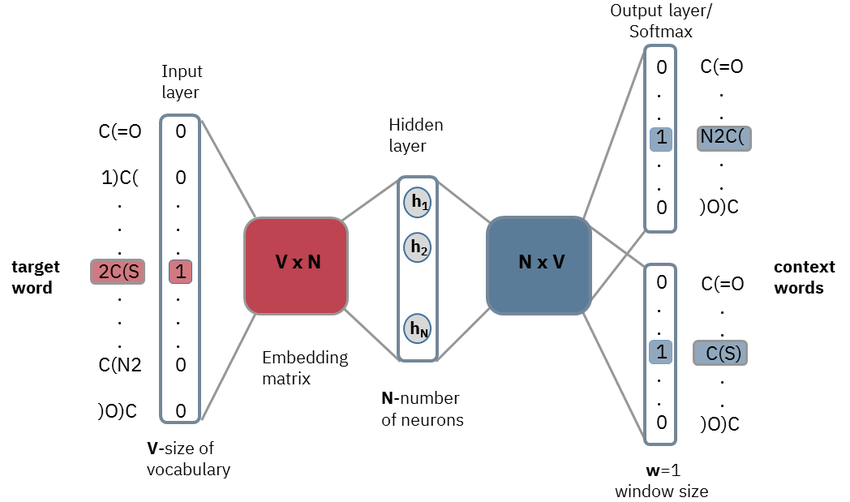
\includegraphics[width=0.7\pdfpagewidth]{images/skipgram.jpg}
        \caption{Esempio di modello Skip-gram}
    \end{figure}
\end{center}

\subsubsection{Addestramento e ottimizzazione}
Durante la fase di addestramento di Word2Vec, l'algoritmo cerca di regolare i parametri in modo che i vettori delle parole riflettano le relazioni semantiche. Questo avviene attraverso l'ottimizzazione di una funzione obiettivo che misura la discrepanza tra le parole reali e quelle previste. L'addestramento avviene attraverso iterazioni multiple su un grande corpus di testi, affinando gradualmente i vettori delle parole.

\subsubsection{Vantaggi e sfide}
Word2Vec ha introdotto importanti vantaggi nel campo del NLP, rendendo possibile la rappresentazione numerica del linguaggio. Questi vettori di parole sono state sfruttati con successo in varie applicazioni NLP, migliorando la comprensione del contesto e la similarità semantica tra le parole. Tuttavia, Word2Vec presenta sfide, come la gestione di parole polisemiche e la cattura di sfumature linguistiche complesse.

\subsubsection{Eredità e avanzamenti successivi}
L'eredità di Word2Vec risiede nell'apertura della strada all'uso di rappresentazioni vettoriali per il linguaggio naturale. L'algoritmo ha ispirato ulteriori sviluppi, come GloVe e i modelli Transformer, che hanno ulteriormente migliorato le prestazioni nell'elaborazione del linguaggio.

\section{I database vettoriali}
Un database vettoriale è una struttura di dati che rappresenta e organizza le informazioni utilizzando vettori matematici. Questi vettori sono spesso utilizzati per rappresentare caratteristiche o attributi di oggetti, consentendo operazioni di ricerca, confronto e analisi efficienti. Questa tecnica trova applicazione in diversi campi, tra cui il trattamento dell'informazione e l'elaborazione del linguaggio naturale (NLP). I database vettoriali offrono vantaggi significativi in termini di velocità e precisione delle ricerche rispetto a metodi tradizionali basati su testo.

\subsubsection{Funzionamento dei database vettoriali}

I database vettoriali operano sulla base della rappresentazione delle informazioni in spazi vettoriali multidimensionali. Ogni elemento nel database è rappresentato da un vettore numerico, dove ogni dimensione del vettore rappresenta un attributo o una caratteristica dell'elemento stesso. L'uso di questa rappresentazione vettoriale consente di misurare la similarità tra elementi attraverso metriche di distanza o somiglianza nello spazio vettoriale.

\subsubsection{Applicazioni nell'NLP e nei LLM}

I database vettoriali sono di fondamentale importanza nell'NLP e nella creazione di Modelli di Linguaggio Basati su LLM come GPT-3. Questi database vettoriali consentono di rappresentare parole, frasi e testi interi in modo che le informazioni semantiche e sintattiche siano catturate nelle relazioni spaziali dei vettori.

Nell'NLP, i database vettoriali sono utilizzati per:
\begin{itemize}
    \item Word Embeddings: La rappresentazione vettoriale delle parole è fondamentale per molte attività, come la classificazione del testo, la traduzione automatica e l'analisi del sentimento.
    \item Recupero dell'Informazione: I vettori consentono il calcolo di similarità semantica tra query e documenti, migliorando il recupero dell'informazione.
    \item Clusterizzazione e Classificazione: I vettori possono essere utilizzati per raggruppare o classificare testi simili basandosi sulle relazioni spaziali.

\end{itemize}

Nei Modelli di Linguaggio Basati su LLM come GPT-3, i database vettoriali contribuiscono all'elaborazione del linguaggio, consentendo di rappresentare contesti, testi di input e testi generati in spazi vettoriali. Ciò consente al modello di comprendere e generare testo coerente, sfruttando le relazioni semantiche tra le parole.

\subsubsection{Database vettoriali famosi}

I realizzatori di db vettoriali sono molti e molti ne sono nati negli ultimi anni, sopratutto dopo l'esplosione di fama di ChatGPT. Tra i più famosi troviamo:
\begin{itemize}
    \item Pinecone: commerciale, che ha costruito intorno al prodotto anche una serie di tool e servizi per l'ingestion dei dati, maggiori informazioni al link \url{https://www.pinecone.io/}
    \item Qdrant: opensource, con una piccola parte di business model riguardante il supporto o l'hosting di un cluster, ha come forza maggiore il suo essere estremamente scalabile, maggiori informazioni al link \url{https://qdrant.tech/}
    \item Chroma: completamente opensource, ha come obiettivo quello di avere un API semplice e che renda la prototipizzazione di un prodotto il più veloce possibile, maggiori informazioni al link \url{https://www.trychroma.com/}
\end{itemize}

\begin{center}
    \begin{figure}[H]
        \centering
        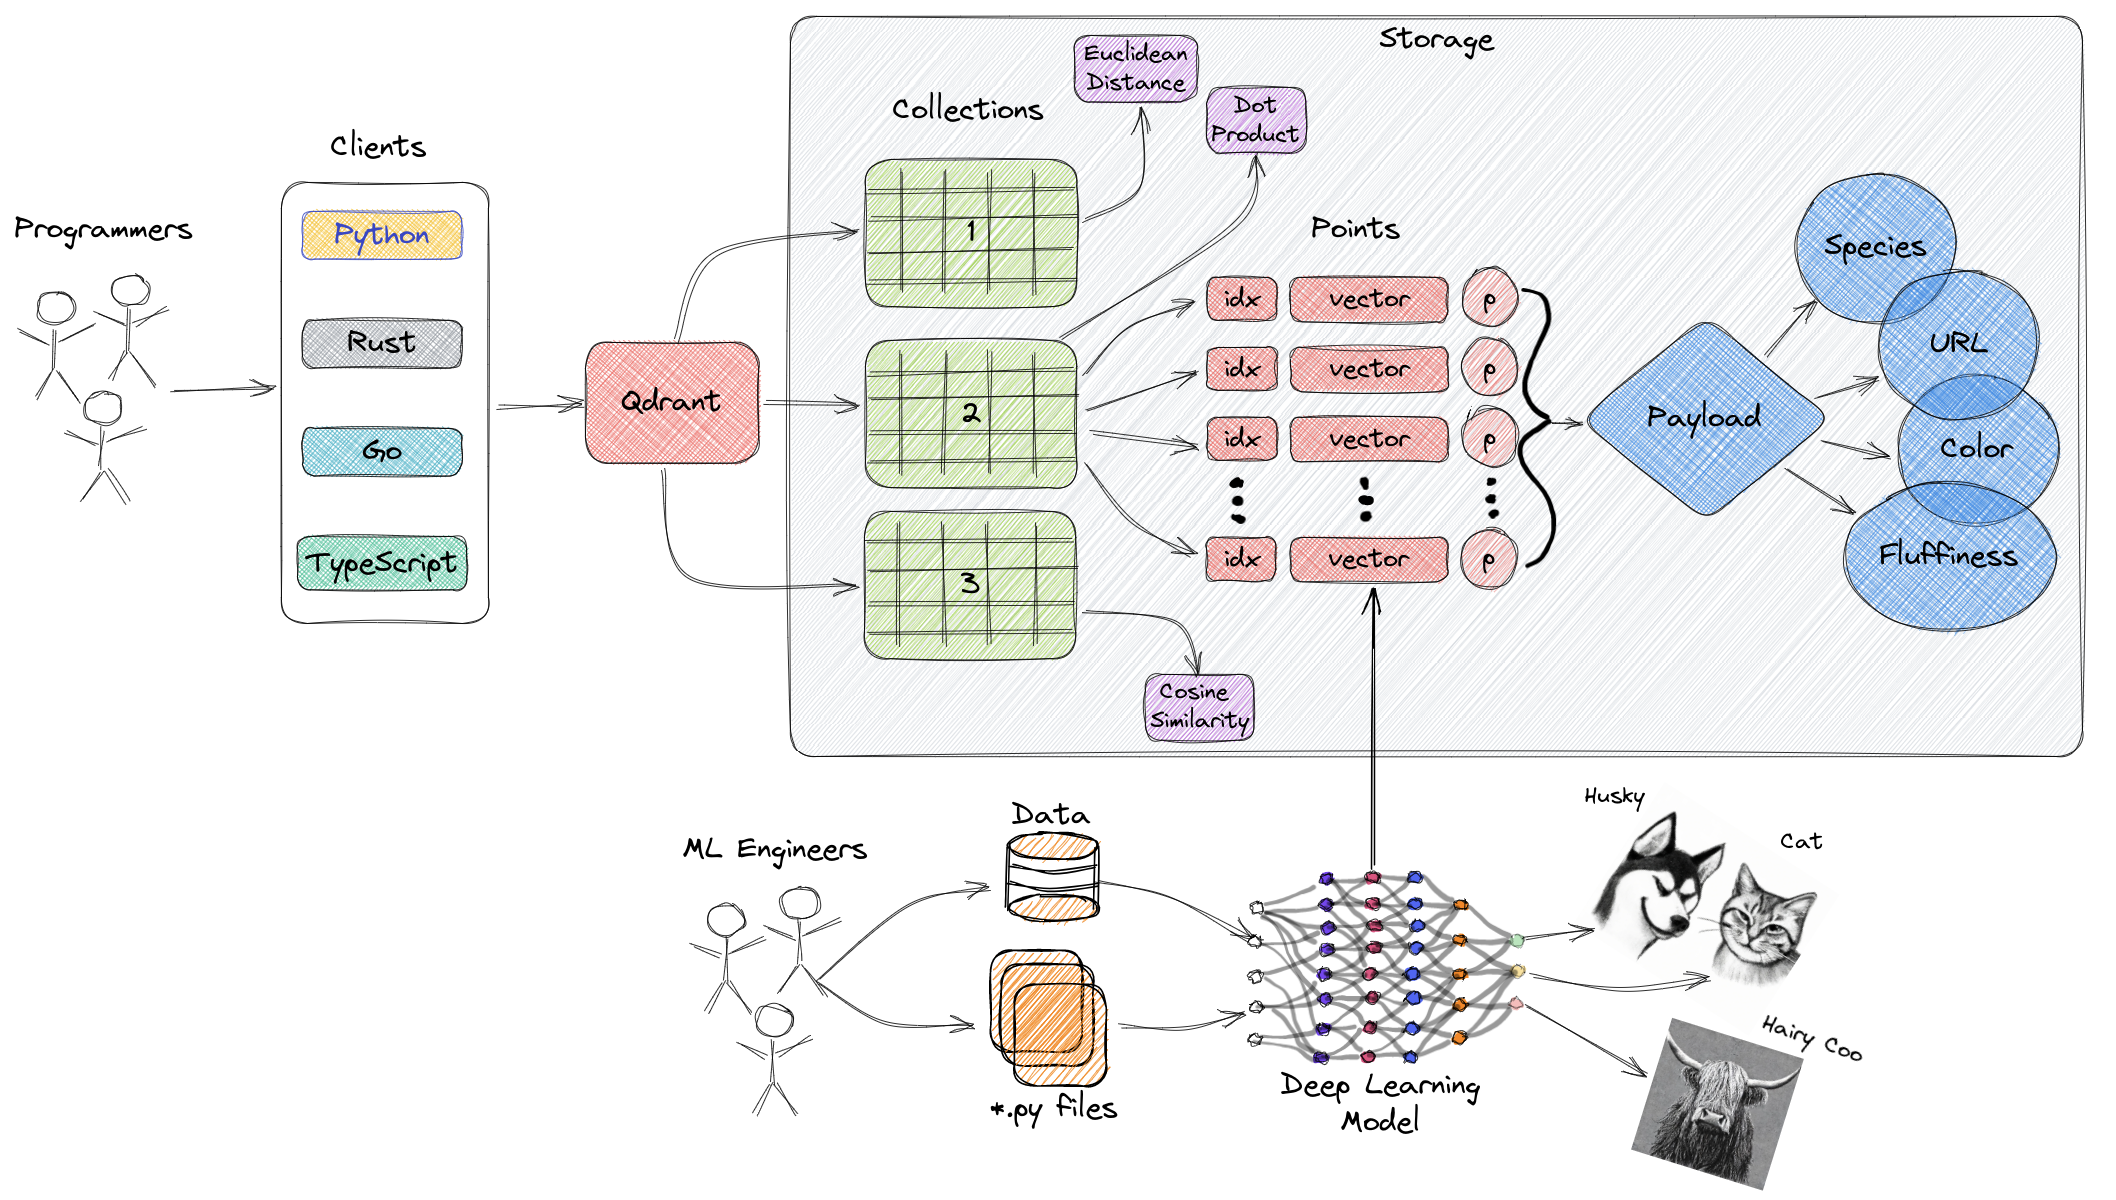
\includegraphics[width=0.7\pdfpagewidth]{images/qdrant_overview.png}
        \caption{Una vista ad alto livello di come è strutturato Qdrant}
    \end{figure}
\end{center}

In conclusione, i database vettoriali sono strumenti essenziali per il trattamento delle informazioni e l'elaborazione del linguaggio naturale. La loro applicazione nei LLM ne potenzia le capacità di comprensione e generazione del testo, contribuendo all'avanzamento delle applicazioni nell'NLP e nei campi connessi.